\begin{enumerate}[label=\thesubsection.\arabic*.,ref=\thesubsection.\theenumi]
\numberwithin{equation}{enumi}

\item
Consider the unity feedback control system in Fig.  \ref{fig:ee18btech11038}. Find the value of K such that $PM = 30\degree$.

\begin{figure}[!ht]
	\begin{center}
		
		\resizebox{\columnwidth}{!}{%\begin{figure}
\tikzstyle{block} = [draw, fill=blue!20, rectangle, 
    minimum height=1cm, minimum width=1cm]
\tikzstyle{sum} = [draw, fill=blue!20, circle, node distance=1cm]
\tikzstyle{input} = [coordinate]
\tikzstyle{output} = [coordinate]
\tikzstyle{pinstyle} = [pin edge={to-,thin,black}]

% The block diagram code is probably more verbose than necessary
\begin{tikzpicture}[auto, node distance=2cm,>=latex']
    % We start by placing the blocks
    \node [input, name=input] {X(s)};
    \node [sum, right of=input] (sum) {};
    
    \node [block, right of=sum] (system) {$G(s)$ };
   
    % We draw an edge between the controller and system block to 
    % calculate the coordinate u. We need it to place the measurement block. 
    
    \node [output, right of=system] (output) {};
    \node [block, below of=system] (measurements) {1};

    % Once the nodes are placed, connecting them is easy. 
    \draw [draw,->] (input) -- node {$U(s)$} (sum);
    \draw [->] (sum) -- node {} (system);
    \draw [->] (system) -- node [name=y] {$Y(s)$}(output);
    \draw [->] (y) |- (measurements);
    \draw [->] (measurements) -| node[pos=0.99] {$-$} 
        node [near end] {} (sum);
\end{tikzpicture}
%\end{figure}}
	\end{center}
\caption{}
\label{fig:ee18btech11038}
\end{figure}
\solution From Fig. \ref{fig:ee18btech11038},
%
\begin{align}
G\brak{s} &= \frac{Ke^{-s}}{s}
\\
H\brak{s} &= 1
\\
\implies 
%
\\
\abs{G\brak{\j\omega_{gc}}H\brak{\j\omega_{gc}}} &= 1
\\
\implies \omega_{gc} &= K  
\end{align}
%
Thus, 
\begin{align}
\label{eq:PM_in_K}
\angle G\brak{\j\omega_{gc}}H\brak{\j\omega_{gc}} &=
 \angle \frac{{Ke^{-jK}}}{jK} 
\\
&= -90\degree - K\brak{\frac{180}{\pi}}
\\
\implies
    PM &= 180\degree -90\degree - K\brak{\frac{180}{\pi}}
\\
 &= 30\degree
    \\
\implies    K&= \frac{\pi}{3}
\end{align}
\item Verify your result by plotting the gain and phase plots of $G\brak{j\brak{\omega}}$ 
\\
\solution The following code plots Fig. \ref{fig:ee18btech11038}

\begin{lstlisting}
codes/ee18btech11038.py
\end{lstlisting}
\begin{figure}[!h]
  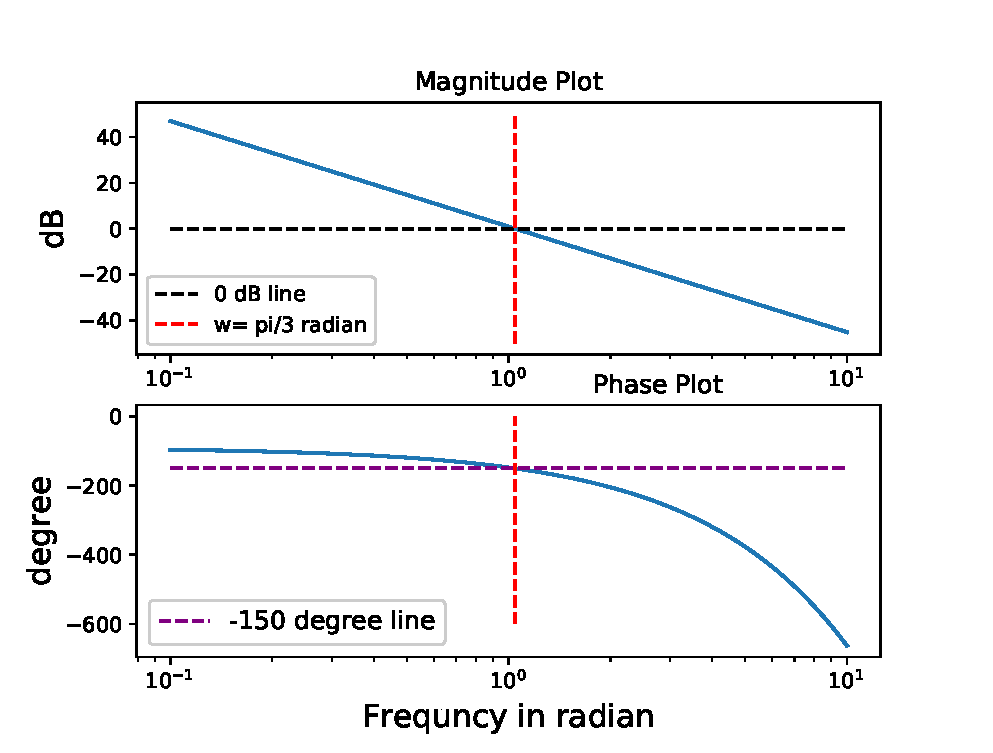
\includegraphics[width=\columnwidth]{./figs/ee18btech11038/ee18btech11038.eps}
  \caption{}
  \label{fig:ee18btech11038}
\end{figure}

\end{enumerate}
